\section{Durchführung}
\label{sec:Durchführung}
Zur Untersuchung der Probenoberfläche wird das \textbf{D8-Labordiffraktormeter} (siehe \autoref{sec:diffraktometer}) verwendet.
Die Röntgenröhre wird mit einer Spannung von $\SI{40}{\kilo\volt}$ und einem Strom von $\SI{35}{\milli\ampere}$ betrieben.
\\
Das Diffraktometer wird über das Programm \textbf{'XRD Commander'} gesteuert.
Der Absorber soll auf 'Auto' eingestellt sein und muss anschließend nicht weiter beachtet werden.
Die Motoren werden über die Eingabemaske, wie in \autoref{fig:commander} zu sehen gesteuert.
\begin{figure}
    \centering
    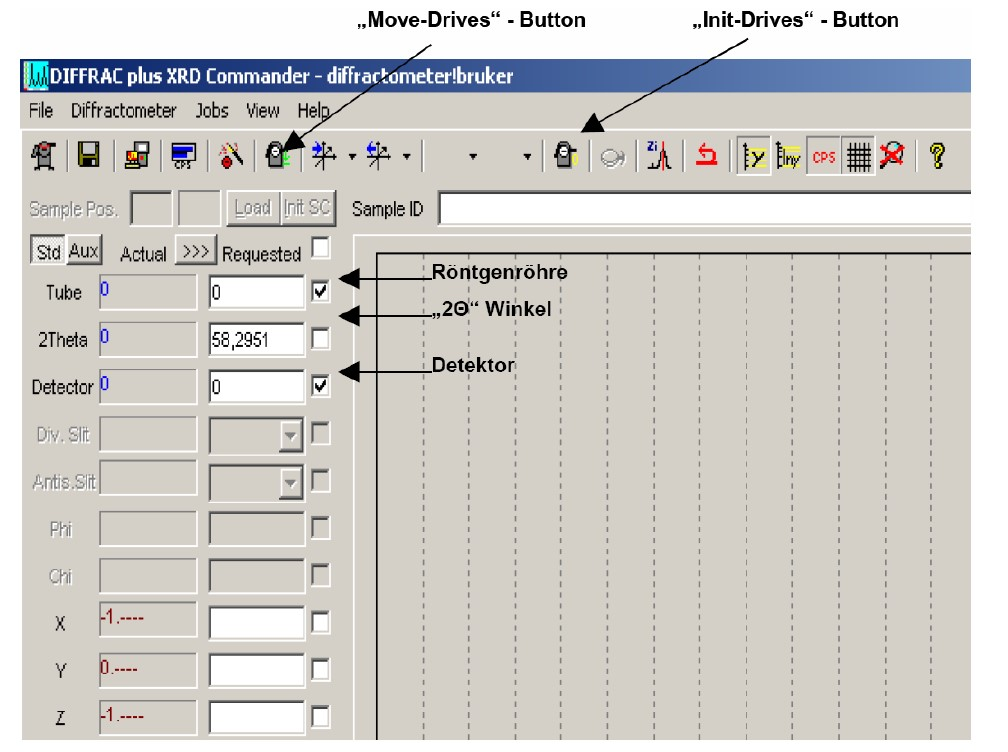
\includegraphics[width=0.7\textwidth]{content/data/xrd_commander.jpg}
    \caption{Ausschnitt des Programms 'XRD Commander' zur Überwachung und Steuerung der Motoren.\cite[3]{anleitung}}
    \label{fig:commander}
\end{figure}
Durch Eintragen der gewünschten Position in das Kästchen und anschließendem setzen des Häkchens, ist nun der Motor ausgewählt und kann über den Button 'Move-Drives' an die ausgewählte Position gefahren werden.
Die Messzeit beträgt $\SI{1}{\second}$ wenn nicht anders angegeben.
\\
\\
Bevor die eigentliche Messung beginnen kann, muss die Probe optimal zwischen Röntgenröhre und Detektor positioniert werden.
Dazu werden drei Messmethoden
\begin{itemize}
    \item Detektorscan
    \item Z-Scan
    \item Rockingscan
\end{itemize}
verwendet, die im folgenden Teil erläutert werden.
Die drei und weitere Messmethoden können über den Reiter 'Scantype' ausgewählt werden.
\\
Zuerst wird der Primärstrahl mithilfe eines \textbf{Detektorscans} justiert, umso die $\SI{0}{\degree}$-Lage des Detektors zu ermitteln.
Dazu muss die Probe aus dem Strahl gefahren werden, indem die z-Koordinnate angepasst wird.
Nun kann der Scan durchgeführt werden, dabei fährt der Detektor mit der Schrittweite $\Delta \theta = \SI{0.02}{\degree}$ in dem Winkelbereich $[\SI{-0.5}{\degree}, \SI{0.5}{\degree}]$ um die Röntgenröhre.
Wie in \autoref{fig:detektorscan_th} dargestellt, folgt die Intensität einer Gaußverteilung.
\begin{figure}[ht]
    \centering
    \begin{minipage}[b]{0.45\linewidth}
      \centering
      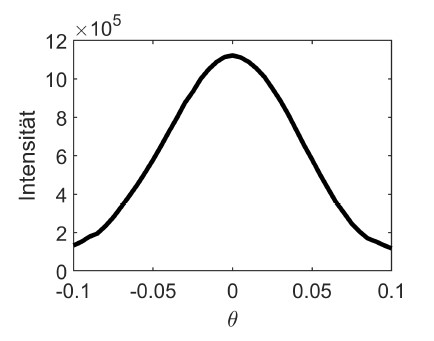
\includegraphics[width=\textwidth]{content/data/detektorscan.jpg}
      \caption{figure}{Intensitätsverteilung für den Detektorscan.\cite[6]{anleitung}}
      \label{fig:detektorscan_th}
    \end{minipage}%
    \begin{minipage}[b]{0.45\linewidth}
      \centering
      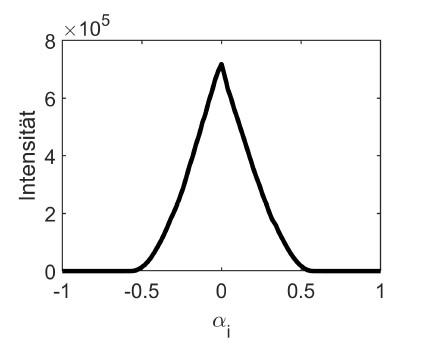
\includegraphics[width=\textwidth]{content/data/rockingscan.jpg}
      \caption{figure}{Intensitätsverteilung für den Rockingscan.\cite[6]{anleitung}}
      \label{fig:rockingscan_th}
    \end{minipage}
\end{figure}
Anschließend wird der Detektor in das Maximum der Verteilung gefahren und kann als neue Nulllage betrachtet werden.
Dazu wird der '$\mathrm{Z}_i$'-Button zur Bestimmung des Peaks betätigt (siehe \autoref{fig:commander}).
In dem sich öffnendem Fenster 'ZI Determination' wird für die theoretische Position Null eingetragen und bestätigt.
Die Probe wird nach Augenmaß über die Schrittmotoren (mit den Koordinaten $X, Y, Z$) zurück in den Stahl gefahren.
\\
\\
Der \textbf{Z-Scan} verschiebt die Probe in der Höhe, wobei bei der optimalen Justage die Probe die hälfte des Strahles abfängt und so die halbe maximale Intensität in den Detektor trifft.
Die Intensitätsverteilung wird im Intervall $[\SI{-1}{\degree}, \SI{1}{\degree}]$ mit Schrittweite $\Delta z = \SI{0.04}{\degree}$ aufgenommen und sollte dem Verlauf der Kurve in \autoref{fig:zscan_th} entsprechen.
\begin{figure}
    \centering
    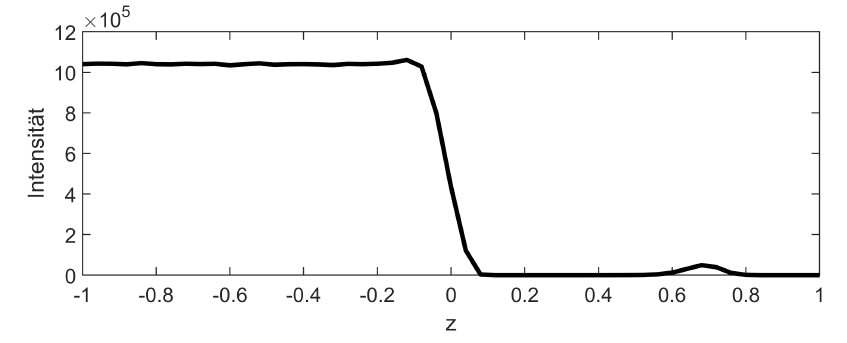
\includegraphics[width=0.6\textwidth]{content/data/zscan.jpg}
    \caption{Intensitätsverteilung für den Z-Scan.\cite[6]{anleitung}}
    \label{fig:zscan_th}
\end{figure}
Nun wird mit einem Doppelklick, auf die Hälfte der maximalen Intensität die $Z$-Position ausgewählt und mit dem 'Move-Drives'-Button angefahren.
Zwar trifft der Strahl die Probe jetzt mit der Intensität $\frac{1}{2}I_\text{max}$, doch vermutlich verläuft der Strahl (wie links in \autoref{fig:rocking_zscan} zu sehen) nicht parallel zur Probe.
\\
\\
Um diese Fehlstellung, also die Verkippung der Probe zu korrigieren wird ein \textbf{Rocking-Scan} durchgeführt.
Bei diesem drehen sich Röntgenröhre und Detektor mit einem konstanten Winkel zueinander ($\alpha_i + \alpha_f = 2 \theta$) um die Probe.
Ebenso kann mit diesem Scan beobachtet werden, ob sich die Probe im Drehpunkt befindet.
Es wird eine Schrittweite von $\Delta \alpha_i = \SI{0.04}{\degree}$ für das Intervall $[\SI{-1}{\degree}, \SI{1}{\degree}]$ und $2 \theta = 0$ gewählt.
\begin{figure}
    \centering
    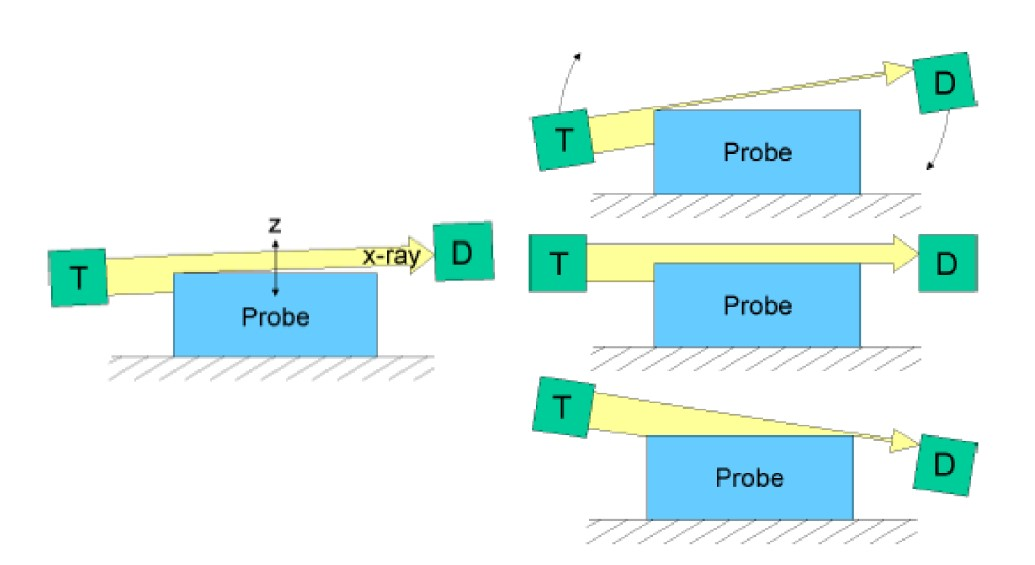
\includegraphics[width=0.7\textwidth]{content/data/rocking_zscan.jpg}
    \caption{Links: Möglicher Strahlenverlauf nach Durchführung des Z-Scans. \\ Rechts: Rocking-Scan zur parallelen Ausrichtung des Strahls zur Probenoberfläche.\cite[5]{anleitung}}
    \label{fig:rocking_zscan}
\end{figure}
Die Intensitätsverteilung soll bei optimaler Justage, wie in \autoref{fig:rockingscan_th} verlaufen und ein symmetrisches Dreieck ergeben.
Wenn dies nicht der Fall ist, wird die $Y$-Koordinate angepasst bis die Asymmetrie verschwindet.
Liegt die maximale Intensität nicht bei $\SI{0}{\degree}$, so muss Röhre und Detektor zum Maximum gefahren werden.
\\
\\
Aufgrund der Justierungen befindet sich die Probe nicht mehr im Intensitätsmaximum des Strahls.
Es wird ein weiterer \textbf{Z-Scan} mit $\Delta z = \SI{0.02}{\degree}$ im Bereich $[-0.5, 0.5]$ durchgeführt, um die Probe wieder in den halben Strahl zu fahren.
\\
Im Anschluss folgt ein zweiter \textbf{Rocking-Scan} unter dem Winkel $2 \theta = \SI{0.3}{\degree}$ im Bereich $[0, 0.3]$ mit der Schrittweite $\Delta \alpha_i = \SI{0.005}{\degree}$.
\\
Ein letzter \textbf{Z-Scan} erfolgt unter dem eingestellten Winkel $2 \theta = \SI{0.3}{\degree}$ um erneut die Position der halben Abschattung zu bestimmen und anzufahren.
Die Messung wird mit der Schrittweite $\Delta z = \SI{0.02}{\degree}$ und (wie bei den vorangegangenen Z-Scans) im Intervall $[-0.5, 0.5]$ durchgeführt.
\\
\\
Die Probe ist nun optimal positioniert und die Reflektivitätsmessung kann beginnen.
Dazu wird der Scantype \textbf{'Omega/2Theta'} und eine Messzweit von $\SI{5}{\second}$ gewählt.
Nun wird bei gleichem Einfallswinkel $\alpha_i$ und Winkel zwischen Probe/Detektor $\alpha_f$ ein Scan mit Schrittweite $\Delta \alpha_i = \SI{0.005}{\degree}$ im Bereich $[\SI{0}{\degree}, \SI{2.5}{\degree}]$ durchgeführt.
\\
Anschließend wird ein 'Diffuser Scan' durchlaufen.
Dieser dient zur Bestimmung des Anteils der gestreuten zur reflektierten Intensität.
Es wird erneut der \textbf{'Omega/2Theta'}-Scan ausgewählt und der Detektorwinkel $\alpha_f$ um $\SI{0.1}{\degree}$ zum Einfallswinkel $\alpha_i$ verschoben.